\begin{figure}[t]
 	\centering
 	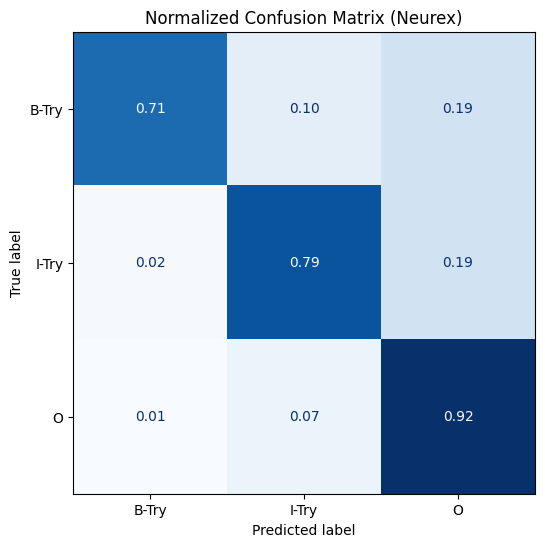
\includegraphics[width=2.4in]{rq2_cm_neurex.png}
        \vspace{-10pt}
 	\caption{Normalized Confusion Matrix --- {\tool} (XState Evaluated As Individual) (RQ2)}
 	\label{fig:rq2-cm-xstate}	
\end{figure}

\begin{figure}[t]
 	\centering
 	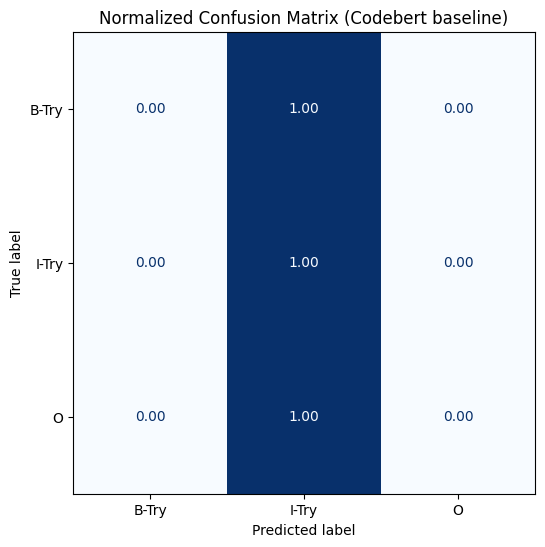
\includegraphics[width=2.4in]{rq2_cm_codebert.png}
        \vspace{-10pt}
 	\caption{Normalized Confusion Matrix --- CodeBERT baseline (XState Evaluated As Individual) (RQ2)}
 	\label{fig:rq2-cm-codebert}	
\end{figure}

To further understand their decision making, we show the confusion matrices for both {\xstate} and the Codebert baseline model. In Figure~\ref{fig:rq2-cm-xstate}, we see {\xstate} has high confidence in predicting statements that are outside try blocks; however, it more often conflates try-block statements with non-try-block statements. Figure~\ref{fig:rq2-cm-codebert} explains why the Codebert baseline model fails the task: It assign the \code{I-Try} label to all the statements. And without the \code{B-Try} label, \code{I-Try} can never be interpreted as a valid try block.